
\section{Architecture Integration}

\subsection{Model Support}

\begin{table}[H]
\centering
\small
\begin{tabular}{llllll}
\toprule
\textbf{Model} & \textbf{Attention class} & \textbf{Nested?} & \textbf{RoPE?} & \textbf{GQA?} & \textbf{Verified} \\
\midrule
DistilBERT & \texttt{MultiHeadSelfAttention} & No & No & No &  \\
RoBERTa & \texttt{BertSelfAttention} (nested) & Yes & No & No &  \\
GPT-2 & \texttt{GPT2Attention} (Conv1D) & No & No & No &  \\
Qwen3.5 & \texttt{Qwen3Attention} & No & Yes & Yes & 0.85 \\
\bottomrule
\end{tabular}
\end{table}

\subsection{Weight Extraction}

\subsubsection{DistilBERT}

\begin{lstlisting}
extracted["q"] = src.q\_lin.weight
extracted["k"] = src.k\_lin.weight
extracted["v"] = src.v\_lin.weight
extracted["o"] = src.out\_lin.weight
\end{lstlisting}

\subsubsection{RoBERTa (nested)}

\begin{lstlisting}
s = src.self
extracted["q"] = s.query.weight
extracted["k"] = s.key.weight
extracted["v"] = s.value.weight
extracted["o"] = src.output.dense.weight
\end{lstlisting}

\subsubsection{GPT-2 (Conv1D)}

\begin{lstlisting}
w = src.c\_attn.weight.t()
q\_w, k\_w, v\_w = w.chunk(3, dim=0)
extracted["q"] = q\_w
extracted["k"] = k\_w
extracted["v"] = v\_w
extracted["o"] = src.c\_proj.weight.t()
\end{lstlisting}

\subsubsection{Qwen (GQA + RoPE)}

\begin{lstlisting}
extracted["q"] = src.q\_proj.weight
extracted["k"] = src.k\_proj.weight
extracted["v"] = src.v\_proj.weight
extracted["o"] = src.o\_proj.weight
\end{lstlisting}

\subsection{GQA Adaptation}

For Qwen-style models where $H_{kv} < H$, the extracted K/V weights are 
adapted:

\begin{lstlisting}
def \_adapt\_to\_kv\_size(weight, bias):
    if weight.shape[0] == self.kv\_head\_size:
        return weight, bias
    if weight.shape[0] \textgreater{} self.kv\_head\_size and weight.shape[0] \% self.kv\_head\_size == 0:
        rep = weight.shape[0] // self.kv\_head\_size
        weight = weight.reshape(self.num\_kv\_heads, rep, -1).mean(dim=1)
        if bias is not None:
            bias = bias.reshape(self.num\_kv\_heads, rep, -1).mean(dim=1).reshape(-1)
    elif weight.shape[0] \textless{} self.kv\_head\_size and self.kv\_head\_size \% weight.shape[0] == 0:
        rep = self.kv\_head\_size // weight.shape[0]
        weight = weight.repeat(rep, 1)
        if bias is not None:
            bias = bias.repeat(rep)
    return weight, bias
\end{lstlisting}

\subsection{SVD Factorization}

Each projection is factorized via:

\begin{lstlisting}
def \_factorize\_and\_set(self, target\_linear, weight, bias=None):
    U, S, Vt = torch.linalg.svd(weight.float(), full\_matrices=False)
    r = min(target\_linear.rank, U.size(1), Vt.size(0))
    sqrt\_S = torch.sqrt(torch.clamp(S[:r], min=1e-5))
    U\_r = U[:, :r] * sqrt\_S.unsqueeze(0)
    V\_r = sqrt\_S.unsqueeze(1) * Vt[:r, :]
    target\_linear.set\_low\_rank\_factors(U\_r, V\_r)
    if bias is not None:
        target\_linear.bias.data.copy\_(bias)
\end{lstlisting}

\subsection{Nested Encoder Handling}

For RoBERTa/BERT, \texttt{is\_nested\_encoder = True}:
\begin{itemize}
\item The output projection is skipped (applied externally).
\item The forward returns the raw context.

\end{itemize}
\begin{lstlisting}
if self.is\_nested\_encoder:
    output = context
else:
    output = self.out\_proj(context)
\end{lstlisting}

\subsection{Injection}

\begin{lstlisting}
def inject\_svd\_linear\_attention(layer, model\_config=None, old\_attn=None, **kwargs):
    target = layer
    cfg = model\_config or target.config
    
    # Nested encoder detection
    is\_nested = hasattr(target, "attention") and hasattr(target.attention, "self")
    if is\_nested and target.attention is old\_attn:
        old\_attn = target.attention.self
    
    new\_attn = SVDLinearAttention(config=cfg, old\_attn=old\_attn, **kwargs)
    new\_attn.is\_nested\_encoder = is\_nested
    
    if is\_nested:
        target.attention.self = new\_attn
    elif hasattr(target, "attention"):
        target.attention = new\_attn
    elif hasattr(target, "self\_attn"):
        target.self\_attn = new\_attn
    elif hasattr(target, "attn"):
        target.attn = new\_attn
    
    return new\_attn
\end{lstlisting}

\subsection{The `step\_recurrent` API}

For streaming inference:

\begin{lstlisting}
def step\_recurrent(self, x\_t, past\_state=None):
    """Process one token.
    
    Args:
        x\_t: [B, d] or [B, 1, d]
        past\_state: (S, Z) from previous step, or None for first step
    
    Returns:
        out\_t: [B, 1, d]
        new\_state: (S, Z)
    """
    # 1. Project, apply feature map
    # 2. Compute decay $\lambda$\_t
    # 3. Update S, Z
    # 4. Compute output
    # 5. Apply out\_proj
    return out\_t, (S\_t, Z\_t)
\end{lstlisting}

\textbf{Usage example:}

\begin{lstlisting}
state = None
for token in sequence:
    out, state = attention.step\_recurrent(token.unsqueeze(0), state)
    # out is the attention output for this token
\end{lstlisting}

\subsection{Failure Modes}

\begin{table}[H]
\centering
\small
\begin{tabular}{lll}
\toprule
\textbf{Failure} & \textbf{Detection} & \textbf{Response} \\
\midrule
Missing projection & \texttt{copy\_weights} raises & Injection aborts \\
Small Frobenius norm & Explicit check & Raises RuntimeError \\
GQA shape mismatch & Explicit reshape & Adapts \\
OOM & RuntimeError & Reduce batch \\
\bottomrule
\end{tabular}
\end{table}

\subsection{Registry}

\begin{lstlisting}
@ATTENTION\_REGISTRY.register("svd\_linear\_attn")
@ATTENTION\_REGISTRY.register("svd\_linear\_attention")
@ATTENTION\_REGISTRY.register("svd\_linear")
class SVDLinearAttention(BaseAttention):
    ...
\end{lstlisting}

\subsection{Causality}

\textbf{Verification.} Gradient of output at position $i$ w.r.t. input at 
position $j > i$ is zero for the causal mode.
\begin{lstlisting}

---
\end{lstlisting}

\begin{figure}[H]
\centering
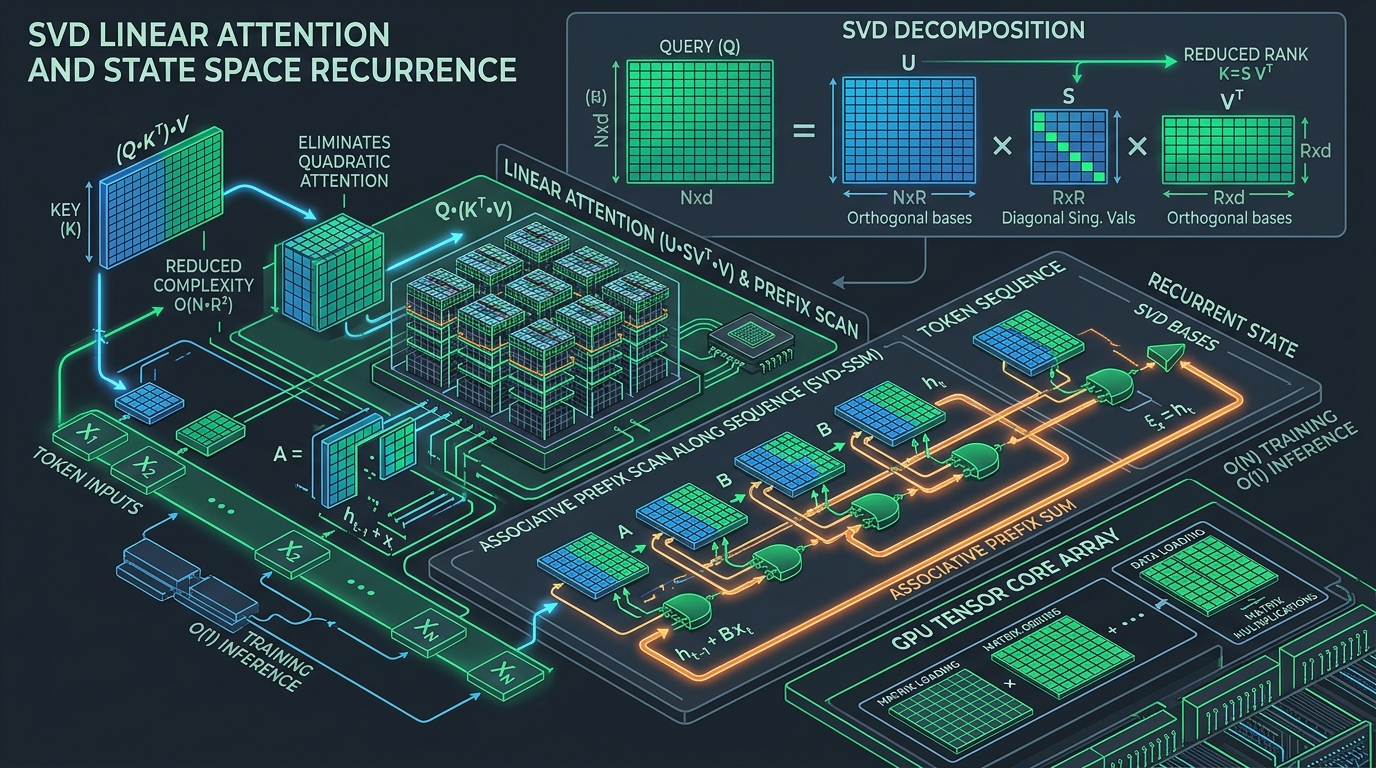
\includegraphics[width=\linewidth]{figures/architecture.jpg}
\caption{High-level architectural diagram of svd\_linear\_attention.}
\label{fig:arch_svd-linear-attention}
\end{figure}

